\scanpage{136}
que $G\unsure{\times|x}V\handwritten{\longrightarrow}V\times V$ est un monomorphisme (c'est le lemme de Nakayama), et on sait bien alors (SGA 3 $\mathrm{VII}_{\mathrm{B}}$ ...) que \deleted{$V$ est un} l'on a un joli quotient $W=V/G$, avec $\deleted{W\quad V}$ $V\handwritten{\longrightarrow}W$ plat et en fait la projection structurale d'un $G_{W}$-torseur. Bien sûr la coalgèbre $\overset{\handwritten{-}}{M}$ n'est autre que celle qui définit le quotient $W$ précédent. En général, il n'est pas question de prouver que $V\handwritten{\simeq}W\times G$ comme variété formelle à opérateurs (i.e. que le torseur précédent est trivial), i.e. de trouver une\deleted{isomorphisme} section de $V$ sur $W$, i.e. un relèvement de comodules $\overset{\handwritten{-}}{M}\handwritten{\longrightarrow}M$; on peut seulement dire que tout relèvement en tant que $k$-vectoriels définira un isomorphisme $A\otimes_{k}\overset{\handwritten{-}}{M}\handwritten{\simeq}M$ de $A$-modules. Cependant, si $G$ est formellement lisse i.e. le dual de $A$ une algèbre de péries formelles (éventuellement à un nb infini de générateurs) alors on aura splittage parfait; ce sera la cas en particulier en car. nulle.

\uline{Exemple} 2. Supposons $A$ commutative pour sa loi d'algèbre. Donc $A$ est l'algèbre affine d'un schéma en monoïdes \inserted{affine} $G$. L'hypothèse sur la filtration coc\deleted{\unsure{c}}omplète est assez étrange ici, elle s'énonce en disant que pour toute $f\handwritten{\in}A$ (fonction sur $G$) \deleted{nulle en $e$}, il existe un entier $n\inserted{\handwritten{\geq\unsure{2|1}}}$ tel que la fonction en $n$\deleted{\unsure{s|x}} variables $f(g_{1}g_{2}\ldots g_{n})$ soit \deleted{identiquement nulle}\inserted{somme de fonctions} à $n-1$ parmi les \unsure{varaables|variables}.\margin{\figure{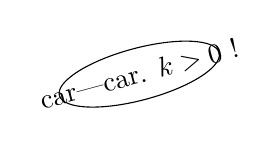
\begin{tikzpicture}[rotate=15,transform shape]
\node[inner sep=3pt] (n) {\handwritten{\unsure{car|car.} $k>0$ !}};
\draw (n.center) ellipse [x radius=1.05cm,y radius=0.33cm];
\end{tikzpicture}}} Si $G$ est de type fini sur $k$\inserted{\handwritten{de car $p>0$}}, je pense que \deleted{dès qu'on y remplace une des variables par $1$, mais alors, faisant tous} cela doit entraîner que \deleted{l'unité de} $G$ est \deleted{point isolé, donc,\deleted{si $G$ est un} \deleted{les arguments \unsure{suffirien|suffirion|suffiront}} comme $G$ est un groupe, que \deleted{groupe, que} $G$ est fini sur $k$. \deleted{Dans dans le cas général, que $G$ est profini sur $k$.} Si $G$ est commutatif (i.e. $\handwritten{\Delta}_{A}$ commutatif), alors le dual de Cartier de $A$ doit être purement infinitésimal, i.e. $G$ doit être unipotent (et réciproquement). On peut conjecturer que \deleted{la con} la condition en question, pour $G$ de type fini pas néc. comm., équivaut à $G$ fini unipotent.}\margin{\handwritten{?}}\inserted{\handwritten{unipotent}} donc si on ne suppose plus nom plus $G$ de type fini, que $G$ est \deleted{\unsure{profini et|profini}} prounipotent.

% archive sheet number: 135
